% !TEX root = ../thesis.tex

\chapter{Introduction}
 \ac{IS} is a fundamental process of fulfilling the information need of individuals by obtaining appropriate information~\cite{savolainen2016elaborating}. In today's society, \ac{IS} plays a crucial role as people regularly engage with various web platforms, such as Google\footnote{\url{https://www.google.com/}}, Youtube\footnote{\url{https://www.youtube.com/}},  ChatGPT\footnote{\url{https://chat.openai.com/}}, etc., to access information from diverse sources based on their specific needs or requirements. These information sources include various formats, including text, audio, video, among others, while the input from users can also take the form of simple text, images, audio, etc. Alazemi~\cite{Alazemi2015UsersIS} has referred to these forms of interaction between individuals and information as information behaviors. Different individuals may interact in \ac{IS} for distinct purposes. Some seek insights to stay informed about current news, social events, entertainment, technology advancements, etc. Meanwhile, others take an active role in seeking precise information to support their critical decision-making processes.

\begin{figure}[h]
	\centering
	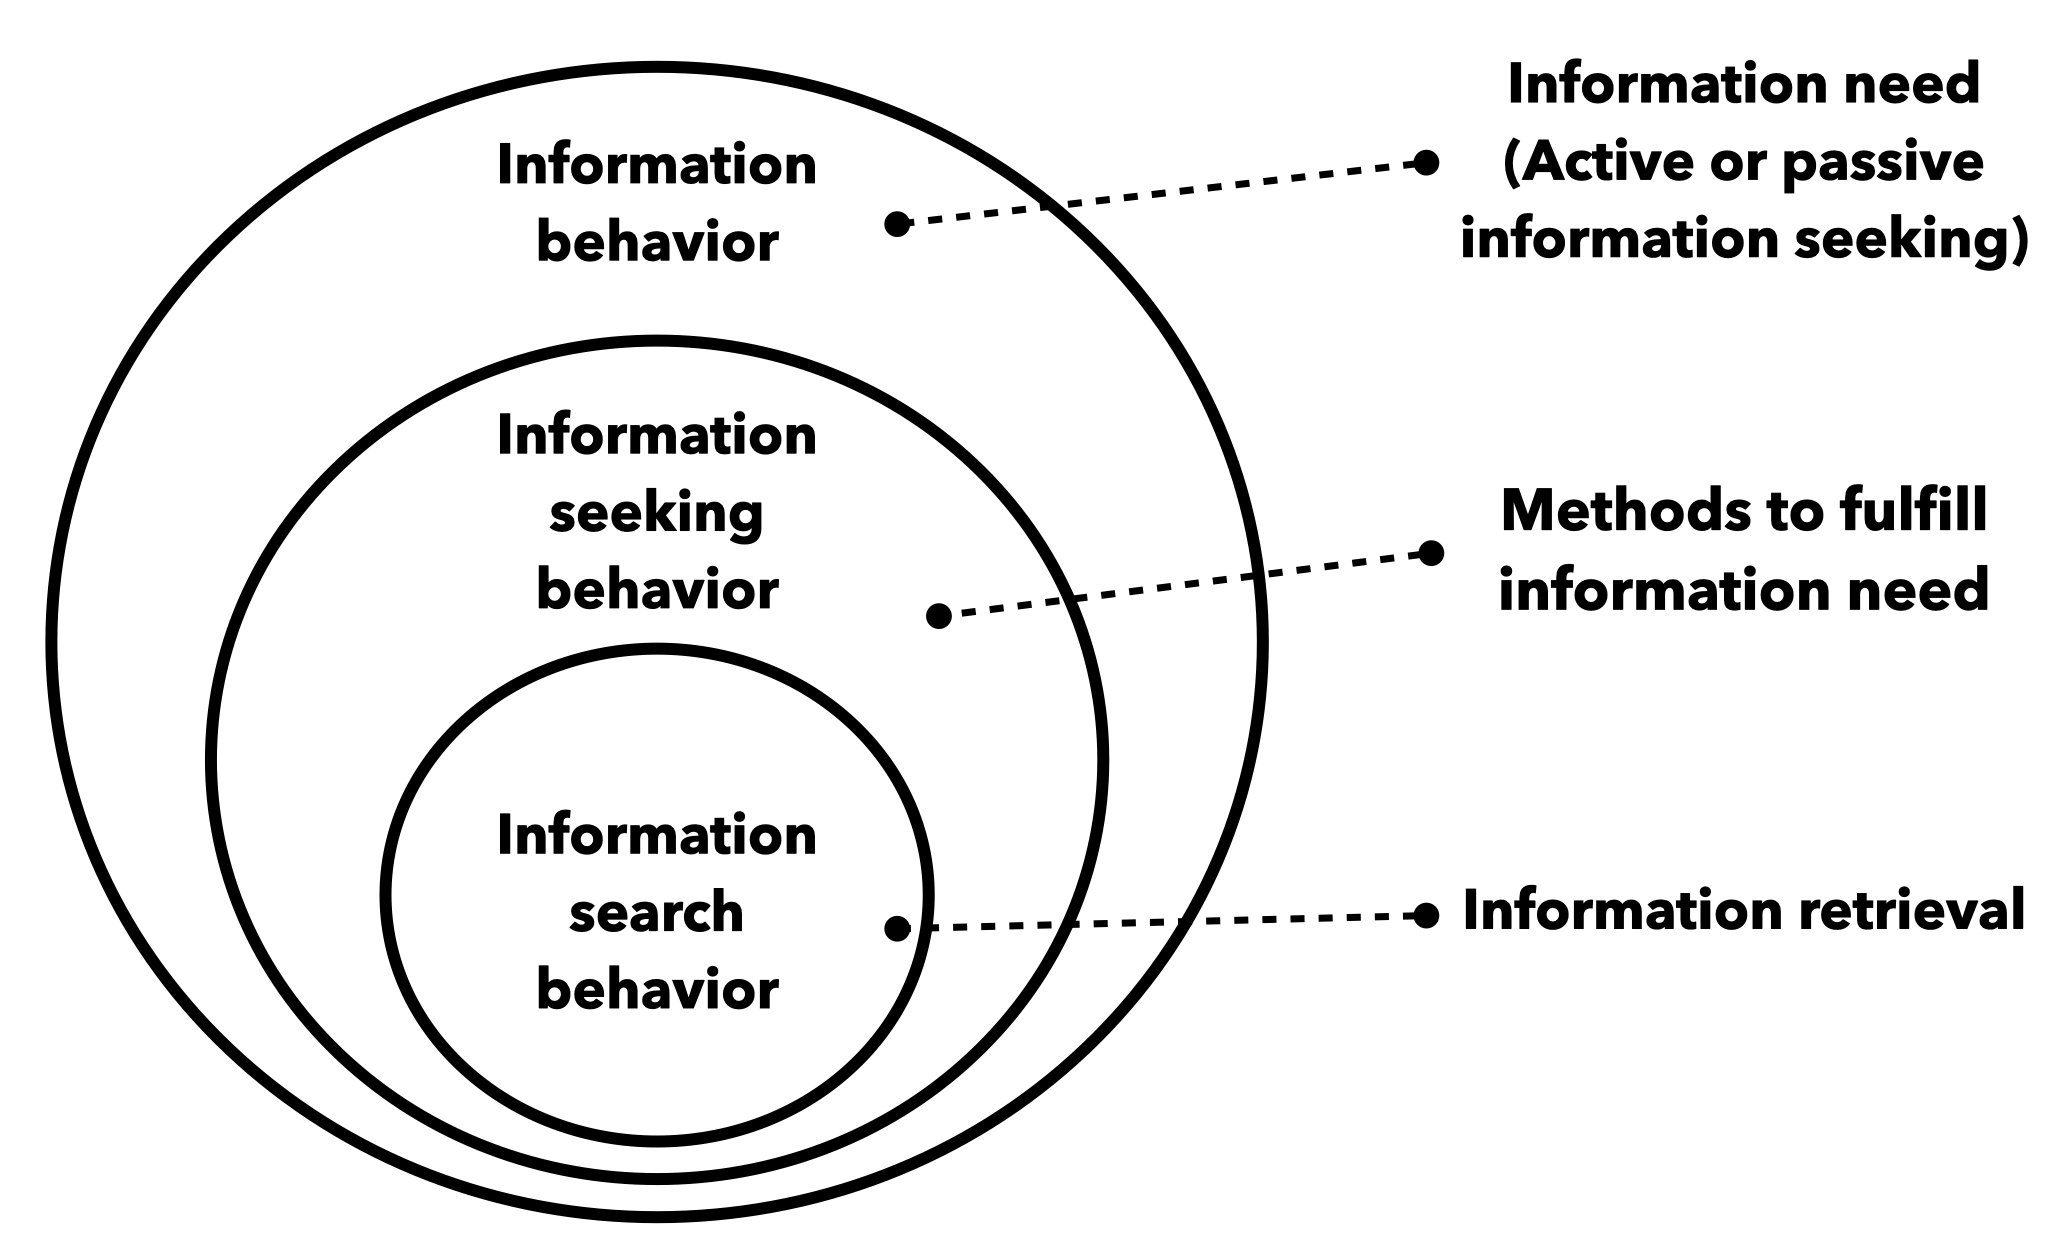
\includegraphics[width=.6\textwidth]{images/thesis_images/information_behaviors.png}
	\caption{Nested model of information behavior~\cite{informationrModelsInformation}. \label{fig:information_behaviors}}
\end{figure} 

Irrespective of whether individuals are active or passive information seekers, they need more information and want to seek information from external sources. Due to the lack of information, users interpret the information gap as a problem and try to manage or resolve this problem by interacting with information sources~\cite{belkin1993interaction}. These user activities are characterized as information seeking behaviors~\cite{belkin1993interaction} and are referred as information search behaviors when seeking the information through a search query. \prettyref{fig:information_behaviors} shows the nested relationship between the different information behaviors, as depicted by Wilson~\cite{informationrModelsInformation}. This depiction highlights that information search behavior is a subset of information seeking behavior, which, in turn, is a subset of information behavior.


In this master thesis, we consider the behaviors related to text interacting information seeking. Furthermore, the thesis is explicitly targeted toward specific and exploratory information-seeking behaviors to understand and help the users in their information-seeking process effectively.

\section{Motivation}

Irrespective of the search platform, the quality of the search results relies on how well the information seekers formulate their information needs. This principle is often referred to by researchers as the "Quality-in quality-out" principle: \textit{A query that more accurately reflects the user's information need will produce better results}~\cite{croft1987i3r}. Consequently, the formulation of the query plays a critical role in the information seeking process. However, assessing the quality of a formulated query can be challenging and is influenced by various factors, including the user's knowledge of their information need, prior search experience, system experience (user interface), and more~\cite{marchionini2007find}.

 \ac{QC} is a widely adopted technique that assists users in formulating their information needs more effectively. \ac{QC} capitalizes on actively indexed data available on the web and leverages query logs generated by millions of users. This technique is commonly observed in modern browsers, offering features such as real-time auto-completion and spelling correction~\cite{bast2006type, gaizauskas1998information}. Studies by Marchionini and White~\cite{marchionini2007find} indicate that information seekers show better engagement in their search activities when using \ac{QC}, resulting in higher levels of user satisfaction. However, even after the query is successfully formulated using \ac{QC}, there are some possible reasons for poor search results (low relevancy)~\cite{azad2019query}. 

\begin{description}
	\item[Cross-domain queries] \hfill \\ These are user queries that span multiple domains or topics, leading to an abundance of false positives. The resolution lies in constructing a well-defined query that aligns with a specific topic based on the information seeker's interest.
	
	\item[Short queries] \hfill \\ When the query length is too short, then the user's information need is not well expressed. A recent analysis to understand the user search queries on 306 million keywords used in google search showed that user queries were comprised of a relatively small number of keywords and the mean keyword length is 1.9 words and 8.5 characters~\cite{google_keyword}. \prettyref{fig:longtail_keywords} provides further insights by examining the distribution of search queries based on their length. It is evident that shorter user queries, indicating weaker intent, are more prevalent compared to longer queries with stronger intent. This pattern namely "Long tail" search queries show the significance of short keyword queries within the user search behavior.
	
	\begin{figure}[h]
		\centering
		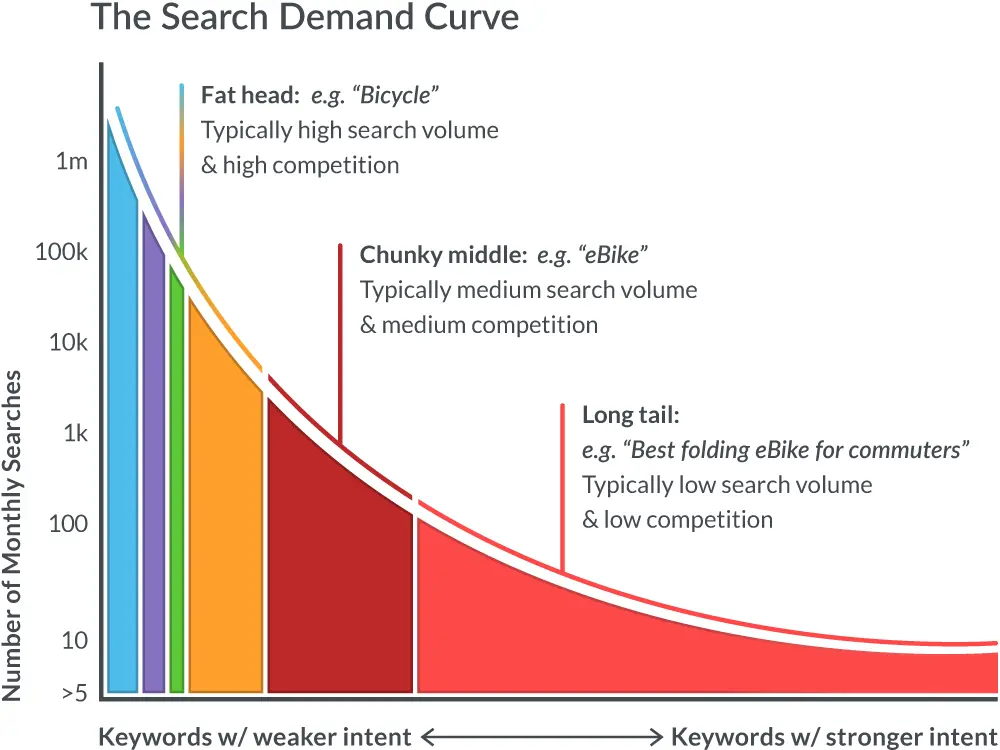
\includegraphics[width=.55\textwidth]{images/outside/search_demand_curve.png}
		\caption[Search query distribution]{Distribution of search queries according to their length~\cite{mozWhatKeywords}. \label{fig:longtail_keywords}}
	\end{figure} 
	
	\item[Poor information needs] \hfill \\ The user is only sure what they are looking for once they see the search results. The user should conduct an exploratory search on a topic and learn from the results.
	
	\item[Poor query formulation] \hfill \\ In this case, users have a clear understanding of what they want to search but struggle to appropriately formulate the search query.
\end{description}

The length of documents in the information source can significantly impact search results. Smaller text documents commonly found in \ac{NLP} projects, such as IMDB reviews and tweets, are typically associated with a single class or topic. Conversely, longer documents like news articles, blogs, e-books, and research papers often contain multiple topics and cannot be logically mapped to a single topic. When such lengthy documents appear frequently in search results, it can result in poor user satisfaction due to their low relevancy (due to the above-mentioned reasons).


To address this issue, users should create well-defined queries that clearly express their intent. For example, a query such as "What are the technological advancements in Robotics related to Unmanned Weapon Systems?" demonstrates a well-formulated query specifying the desired information. However, demanding users to consistently provide such specific queries can be challenging, particularly in exploratory tasks where users may be uncertain about what they are searching for. Additionally, this approach may lead to a sub-optimal search experience, as it restricts users to only certain types of queries.

Rather than expecting users to consistently formulate precise queries, an alternative approach is to guide them using interactive relevance paths derived from a simple user query. These relevance paths are representations of documents extracted from the top retrieved documents for the original query. This methodology is rooted in the concept of "Content-driven information seeking"~\cite{marchionini2007find}, which assumes that the top documents are relevant to the query. Research findings suggest that content-driven relevance paths offer benefits for both exploratory searches and known-item searches~\cite{marchionini2007find}. Particularly when dealing with long text documents, these content-driven interfaces can assist users in narrowing down the search space and finding relevant documents more efficiently. To help users with highly heterogeneous topics within search results, this master thesis proposes an effective and unsupervised topic extraction technique from the top search results.
 
\section{Research Questions}

\ac{IE} and \ac{IR} are two highly effective techniques used in research to fulfill user information needs. \ac{IE} refers to the automated extraction or mining of specific information from data, while IR focuses on retrieving relevant documents for a given user query. Gaizauskas and Wilks~\cite{gaizauskas1998information} have emphasized the complementary nature of these techniques and highlighted the potential for creating practical and robust tools by combining them. For instance, \ac{IE} can aid in formulating the user's information need more accurately, while IR can facilitate the retrieval of high-quality search results.
 
This master thesis introduces an interactive system that integrates both \ac{IE} and \ac{IR} techniques to effectively meet user information needs. The thesis presents an unsupervised soft clustering approach designed to model documents in multiple languages as a mixture of sub-topics. These sub-topics are extracted using deep intrinsic information derived from keywords. The evaluation of this approach is conducted in three phases, including not only the assessment of clustering using various evaluation metrics but also a user satisfaction survey. The research questions (RQ) detailed below specifically address the evaluation of the proposed approach.

\begin{enumerate}
\item[RQ1:] How effective is the sub-topic modeling approach in creating distinctive clusters from long text documents?

Clustering algorithms generate topics (well-formed clusters) from a collection of documents. However, these topics become highly valuable to users when they exhibit distinctiveness especially in the case of news-articles. The presence of heterogeneous clusters enables users to easily identify relevant documents related to both the query and the sub-topic cluster. To generate such highly distinctive clusters, a candidate keyword selection approach is introduced and evaluated. This research question aims to assess the effectiveness of the keyword selection technique when combined with conventional clustering. Both intrinsic and extrinsic clustering evaluation techniques and a survey are chosen to evaluate the clustering output. The parameters of the clustering pipeline are fine-tuned using these evaluation metrics and manual observation.



\item[RQ2:] How can the retrieved documents be effectively represented for a given user query and sub-topic?  \\

When users select a specific sub-topic cluster, it is assumed that the retrieval results relevant to both the user query and the chosen sub-topic are presented to the user. In this master thesis, two distinct  \ac{IR} systems are proposed to retrieve documents relevant to the user query and the selected sub-topic. The objective of this research question is to compare these two \ac{IR} systems and determine the better system. A survey is performed, and the collected data is analyzed to answer the RQ2. Survey participants have the opportunity to read the retrieved documents from both \ac{IR} systems and respond to five questions. A statistical test is performed on the survey data to determine whether the results from the two \ac{IR} systems exhibit any significant differences. Further details regarding the  \ac{IR} systems and survey questions are provided in subsequent sections of the report.


\item[RQ3:] What is the impact of sub-topic and document rankings on the identification of positive documents from the candidate pool? \\

Displaying only documents related to a specific sub-topic can restrict users from accessing all relevant retrieved results for a given query. This research question addresses the impact of the sub-topic clustering output to find the positive documents against the baseline approach. An exploratory precision analysis is conducted to evaluate this impact. Additionally, this research question aims to extract valuable insights from the clusters and their rankings. For instance, \textit{Does a particular sub-topic cluster ranking yield higher precision compared to the baseline?} To address this research question, the widely used \ac{IR} evaluation metric, \ac{MAP}, is used for ranking analysis. Furthermore, the proposed approach's retrieval performance is compared to the literature.

\end{enumerate}


\section{Thesis Structure}

This master thesis is structured into seven chapters, spanning from Chapter 2 to Chapter 8. Chapter 2 delves into the problem context, emphasizing the problem statement. In Chapter 3, essential technical information and background are provided to facilitate comprehension of the selected technologies used in implementing the proposed methodology. Following that, Chapter 4 comprehensively examines the relevant literature that relates specifically to the master thesis. Chapter 5 outlines the proposed approach in detail. Subsequently, Chapter 6 illustrates the experiment setup, while Chapter 7 presents the experiment results. Finally, in Chapter 8, critical aspects of the thesis are highlighted, including an overview of the limitations and suggestions for future work.



